\chapter{実験}
\label{chap:実験}

本章では，実験条件と評価方法を記述する．
モデル構成や損失関数の詳細は第\ref{chap:proposed_method}章で示しているため，
本章では再現可能性に関わる設定を中心に整理する．
具体的には，以下の三点を扱う．
\begin{enumerate}
  \item[(i)] 埋め込みモデルの比較（主成分分析（PCA）による可視化を含む）
  \item[(ii)] 対照学習の実験設定と評価指標
  \item[(iii)] 強化学習の実験設定と評価指標
\end{enumerate}
各実験の結果は第\ref{chap:結果}章で示す．

\section{埋め込みモデルの比較}
\label{sec:embedding_experiment}

本研究では，オノマトペの意味埋め込みとして Sarashina \cite{sarashina} と
SigLIP \cite{siglip} の 2 種類を比較する．
各オノマトペ $w$ をテンプレート文に埋め込み，
\begin{center}
  \texttt{「<w>と歩いている．」}（ただし $w=\text{通常}$ のときは「普通に歩いている．」）
\end{center}
からテキスト埋め込み $u_{\mathrm{sem}}$ を得る．
得られた埋め込みは L2 正規化し，後段の対照学習で利用する．

\subsection{主成分分析（PCA）による可視化}
\label{subsec:embedding_pca}

埋め込みの幾何的構造を確認するため，PCA により 2 次元へ射影して可視化する．
11 語の fine ラベルに加えて，4 グループの coarse ラベルでも色分けし，
同一ラベルが近傍に配置されるかを確認する．
この可視化により，埋め込みモデルごとの「意味的分離性」や
類似語間の距離感（例：速い系／遅い系の分離）を定性的に評価する．

\section{対照学習の実験}
\label{sec:contrastive_experiment}

対照学習は Phase 1（\ref{sec:offline_phase}）に従って実施し，
MotionCLIP \cite{MotionCLIP} の潜在空間とテキスト埋め込みの整合を学習する．
本節では，実験条件，評価指標，および潜在空間における速度情報反映の補助評価を記述する．

\subsection{比較条件}
\label{subsec:contrastive_conditions}

損失関数は SupCon \cite{supcon} を用い，MotionCLIP の motion 埋め込みとテキスト埋め込みの
コサイン類似度に基づく対照損失を最小化する．同時に，VAE による系列再構成損失を併用し，
意味整合（検索指標の改善）と運動再構成の両立を図る．

学習は freeze/full の 2 段階で行い，前段階で得られた最良モデルを次段階の初期値として引き継ぐ．
クラス不均衡への対策として WeightedRandomSampler を用い，バッチ内に各ラベルが
概ね均等に含まれるよう調整する．

\subsubsection{学習手順}
\label{subsubsec:contrastive_procedure}

学習・評価は以下の流れで実施する．
\begin{enumerate}
  \item \textbf{データ分割}: 乱数シード（seed）を固定して学習・検証・評価集合に分割し，
    探索では seed を変えた複数分割で評価する．
  \item \textbf{freeze 学習}: encoder を凍結し，テキスト側（および出力ヘッド等）のみ更新して
    2000 steps 学習する．
  \item \textbf{full 学習}: freeze の最良重みを初期値として読み込み，encoder を含めて
    8000 steps 学習する．
  \item \textbf{モデル選択}: 評価間隔 200 steps ごとに検証集合の $\mathrm{avg\_r@1}$ を算出し，
    最大値を与える重みを最良モデルとして採用する．
  \item \textbf{集約}: 同一条件（$\tau,\lambda_{\mathrm{vae}},\lambda_{\mathrm{con}}$）について
    seed を変えた複数試行の評価指標を集約し，mean$\pm$std を算出する．
\end{enumerate}

この二段構成（freeze$\rightarrow$full）により，まずテキスト側のプロトタイプを安定化させた上で，
motion encoder を含む潜在空間全体を微調整する．

\subsection{最終設定}
\label{subsec:contrastive_final_setup}

Optuna の探索結果を踏まえ，本研究の最終実験では freeze$\rightarrow$full の 2 段階学習を実施した．
freeze 段階は 2000 steps，full 段階は 8000 steps とし，full は freeze の重みを初期値として引き継ぐ．
また，再現性を確認するため乱数シード（seed）を変えて複数回学習し，結果は seed 間平均（mean$\pm$std）で報告する．

\begin{table}[H]
  \centering
  \caption{対照学習の実験プロトコル（固定条件）}
  \label{tab:contrastive_setup}
  \begin{tabular}{ll} \toprule
    \textbf{項目} & \textbf{設定値} \\ \midrule
    ラベル粒度    & 11ラベルのオノマトペ \\
    意味埋め込み  & Sarashina \\
    損失関数      & SupCon+ VAE \\
    バッチサイズ  & 32 \\
    学習率スケジューラ & ReduceLROnPlateau（監視指標: $\mathrm{avg\_r@1}$） \\
    評価間隔      & 200 steps \\
    最良モデル選択& $\mathrm{avg\_r@1}$ 最大 \\
    学習ステップ  & freeze: 2000 / full: 8000 \\
    乱数シード（seed） & 41, 42, 43 \\
    スイープ対象  & $\tau,\ \lambda_{\mathrm{vae}},\ \lambda_{\mathrm{con}}$ \\ \bottomrule
  \end{tabular}
\end{table}


\subsection{評価指標}
\label{subsec:contrastive_metrics}

意味整合の度合いは，検索再現率（R@K）で評価する．
以下では，Text$\rightarrow$Motion を t2m，Motion$\rightarrow$Text を m2t と表記する．
両方向の指標は，
\begin{align}
  \mathrm{R@}K
  = \frac{1}{N}\sum_{i=1}^{N}\mathbf{1}\!\left[\mathrm{rank}_i \le K\right]
\end{align}
で定義する．

再構成誤差は MPJPE 風の平均 L2 距離で評価する．
2D 系列 $X=\{x_{t,j}\}$，再構成 $\hat{X}=\{\hat{x}_{t,j}\}$ に対し，
\begin{align}
  \mathrm{MPJPE}
  = \frac{1}{T J}\sum_{t=1}^{T}\sum_{j=1}^{J}\left\|x_{t,j}-\hat{x}_{t,j}\right\|_2
\end{align}
と定義する．

加えて，潜在空間の分離度はシルエット係数で評価する．
サンプル $i$ の同一クラス平均との差を $a_i$，
異クラスのうち平均距離が最小となる値を $b_i$ とすると,
\begin{align}
  s_i = \frac{b_i - a_i}{\max(a_i, b_i)},\quad
  \mathrm{Sil} = \frac{1}{N}\sum_{i=1}^{N}s_i
\end{align}
で定義される．
これらにより，動作系列の復元精度と意味整合の両面から性能を確認する．

\subsection{潜在空間における速度情報の反映評価}
\label{subsec:contrastive_speed_reflection_eval}

対照学習の損失関数は速度を直接教師としない．
しかし，オノマトペの意味には速度差が暗に含まれるため（例：「せかせか」は速く，「のろのろ」は遅い），
対照学習の結果として潜在空間に速度情報が反映される可能性がある．
この仮説を定量的に検証するため，
同一サンプル集合（$N=284$）に対して，本研究で最終採用した設定
（\ref{subsec:contrastive_final_setup}）のみを対象に評価を行う．
第\ref{chap:結果}章では，この best model に対する結果を示す．

HOYO データセットは 2D 関節座標であり，3D 空間の歩行速度の真値は得られない．
そこで，各フレームにおける頭部関節と両足中点のユークリッド距離を見かけ高さ $h_t$ として定義する．
\begin{align}
  h_t = \left\| p^{(\mathrm{head})}_t - \frac{p^{(\mathrm{lfoot})}_t + p^{(\mathrm{rfoot})}_t}{2} \right\|_2
\end{align}
カメラに接近するほど $h_t$ は増大するため，その時間変化率は接近速度の代理指標として利用できる．
外れ値除去と平滑化を施した後，対数高さ系列 $\log \bar{h}_t$ の時間 $t$ [s] に対する
最小二乗直線の傾き $\hat{a}_n$ を求め，速度代理指標を
\begin{align}
  v_{\mathrm{scale},n} = \max(0,\, \hat{a}_n)
\end{align}
で定義する．
なお，本指標は 2D 画像座標上の見かけの接近速度であり，絶対歩行速度とは異なる．
前処理パラメータおよび導出の詳細は付録\ref{sec:appendix_speed_proxy}に示す．

潜在空間から速度情報をどの程度復元できるかを，回帰と分類の 2 つの観点で評価する．
\begin{itemize}
  \item \textbf{回帰評価}：
  標準化した潜在ベクトルを入力，$v_{\mathrm{scale}}$ を目的変数として，
  Ridge 回帰（$\alpha=1.0$）を 5-fold out-of-fold（OOF）で適用する．
  指標は Spearman $\rho$，$R^2$，MAE とする．
  \item \textbf{分類評価}：
  $v_{\mathrm{scale}}$ を 3 分位で low/mid/high に離散化し，
  クラス不均衡を補正したロジスティック回帰を同様に 5-fold OOF で適用する．
  指標は macro-F1 と balanced accuracy とする．
\end{itemize}

偶然一致の影響を除外するため，回帰の Spearman $\rho$ と分類の macro-F1 に対して
それぞれ 1000 回の置換検定を実施する．
本研究では，次の 3 条件を同時に満たす場合を「速度情報反映が成立」と判定する．
\begin{enumerate}
  \item $\rho \ge 0.35$（中程度の効果量 \cite{Cohen1988}）
  \item macro-F1 $\ge 0.50$（3 クラスのランダム期待値 $\approx 0.33$ を上回る水準）
  \item $p < 0.05$
\end{enumerate}

対照学習の実験結果は，第\ref{chap:結果}章で報告する．

\section{強化学習の実験}
\label{sec:rl_experiment}

Phase 2 の実験では，Isaac Lab 上の H1 ヒューマノイドに対して
PPO を用いたスタイル条件付き歩行方策を評価する．
本節では，比較対象，評価プロトコル，および指標定義を記述する．

\subsection{比較対象と評価プロトコル}
\label{subsec:rl_protocol}

比較条件と評価条件を表\ref{tab:rl_comparison_runs}に示す．
以下では，スタイル追従項に付与する重みを「スタイル重み」と呼ぶ．

\begin{table}[htb]
  \centering
  \caption{強化学習比較で用いた条件と評価設定}
  \label{tab:rl_comparison_runs}
  \small
  \begin{tabular}{lll} \toprule
    \textbf{条件 ID} & \textbf{スタイル重み} & \textbf{速度条件} \\ \midrule
    A & 0.0 & $v_x^{\mathrm{cmd}}=0.5$ \\
    B & 2.0 & $v_x^{\mathrm{cmd}}=0.5$ \\
    C & 4.0 & $v_x^{\mathrm{cmd}}=0.5$ \\
    D & 6.0 & $v_x^{\mathrm{cmd}}=0.5$ \\
    \bottomrule
  \end{tabular}
\end{table}

主比較では，条件間の差をスタイル重みのみに限定するため，
速度指令値を $v_x^{\mathrm{cmd}}=0.5$ に固定した．
条件 ID は，スタイル重みの昇順（0.0, 2.0, 4.0, 6.0）に対応して A～D を付与した．
さらに，スタイル報酬なし条件でもスタイル関連指標を算出可能な設定で評価した．

\subsection{環境および学習パラメータ}
\label{subsec:rl_setup}

シミュレーションおよび学習の主要パラメータを表\ref{tab:rl_hyperparams}に示す．

Phase 1 の MotionCLIP エンコーダは凍結して用いる．

\begin{table}[htb]
  \centering
  \caption{シミュレーション環境および PPO のハイパーパラメータ}
  \label{tab:rl_hyperparams}
  \begin{tabular}{lc} \toprule
    \textbf{項目}  & \textbf{設定値} \\ \midrule
    シミュレータ   & Isaac Lab       \\
    ロボットモデル & H1 Humanoid     \\
    学習環境数     & 2048            \\
    評価環境数     & 16              \\
    制御周期       & 50 Hz           \\
    エピソード長   & 20 s            \\
    アルゴリズム   & PPO (On-policy) \\
    \bottomrule
  \end{tabular}
\end{table}

\subsection{使用ロボットH1の詳細}
\label{subsec:h1_robot_detail}

本研究で用いるロボットは，Isaac Lab の Unitree H1 である．
制御入力は 19 次元の関節位置指令であり，
左右脚（hip yaw/roll/pitch, knee, ankle），体幹（torso），
左右腕（shoulder pitch/roll/yaw, elbow）を含む．
また，シミュレーション刻みは $\Delta t=0.005$\,s，decimation は 4 であるため，
方策の制御周期は 50\,Hz となる．

スタイル評価では，H1 の 3D リンク位置を HOYO 互換の 14 関節へマッピングし，
$Y_{\mathrm{H1}} \to x_{\mathrm{HOYO}},\ -Z_{\mathrm{H1}} \to y_{\mathrm{HOYO}}$
の座標変換を適用する．
H1 に明示リンクがない頭部・手先は，torso/elbow 基準のオフセットで補完する．

\begin{figure}[H]
  \centering
  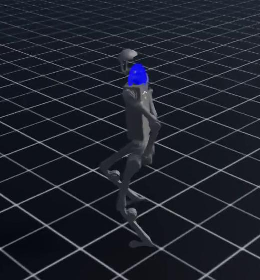
\includegraphics[width=0.40\linewidth]{figs/4/h1_standing_sim.pdf}
  \caption{強化学習環境における H1}
  \label{fig:h1_standing_sim}
\end{figure}

\subsection{報酬設定}
\label{subsec:rl_rewards}

報酬はタスク項・スタイル項・正則化項で構成する．
比較実験で用いた主要項（Task/Style）を表\ref{tab:reward_main}に，
正則化項を表\ref{tab:reward_reg}に示す．
スタイル追従項の重みのみ条件ごとに変更し（0.0/2.0/4.0/6.0），
$\beta_{\mathrm{text}}=0.0$，$\beta_{\mathrm{teach}}=1.0$ を共通設定とした．

\begin{table}[H]
  \centering
  \caption{主要報酬項（Task/Style）}
  \label{tab:reward_main}
  \footnotesize
  \setlength{\tabcolsep}{4pt}
  \begin{tabular}{>{\raggedright\arraybackslash}p{0.46\linewidth} >{\raggedright\arraybackslash}p{0.34\linewidth} c} \toprule
    \textbf{Reward Term (English, NaVILA-aligned)} & \textbf{Symbol / Eq.} & \textbf{Weight} \\ \midrule
    Linear Velocity Tracking (XY) & $\phi_{\mathrm{lin},t}$ (\eqref{eq:task_track_lin}) & $0.5$ \\
    Heading Tracking (World Yaw) & $\phi_{\mathrm{head},t}$ (\eqref{eq:task_track_heading}) & $0.2$ \\
    Style Tracking (Text/Teach) & $r_{\mathrm{style},t}^{\mathrm{raw}}$ (\eqref{eq:rl_style_raw}) & 条件依存 \\ \bottomrule
  \end{tabular}
\end{table}

\begin{table}[H]
  \centering
  \caption{正則化項（比較条件間で固定）}
  \label{tab:reward_reg}
  \footnotesize
  \setlength{\tabcolsep}{4pt}
  \begin{tabular}{>{\raggedright\arraybackslash}p{0.72\linewidth} c} \toprule
    \textbf{Reward Term} & \textbf{Weight} \\ \midrule
    Action Rate Penalty & $-0.005$ \\
    Joint Accelerations & $-1.25 \times 10^{-7}$ \\
    Joint Torques (Energy Proxy) & $0$ \\
    Angular Velocity Penalty (XY) & $-0.05$ \\
    Feet Air Time & $0.25$ \\
    Feet Slipping Penalty & $-0.25$ \\
    Feet Stumble Penalty & $-0.5$ \\
    Flat Orientation & $-1.0$ \\
    DOF Position Limits Penalty & $-1.0$ \\
    Joint Deviation (Hip) & $-0.05$ \\
    Joint Deviation (Arms) & $-0.05$ \\
    Joint Deviation (Torso) & $-0.02$ \\
    Termination Penalty & $-200.0$ \\ \bottomrule
  \end{tabular}
\end{table}

\noindent\textit{注記}：報酬項名は NaVILA 原論文を基準に統一し，
H1 拡張項（Style Tracking, Heading Tracking, DOF 制約など）は本研究設定として追加した．

\noindent スタイル重みの候補値は $\{0.0, 2.0, 4.0, 6.0\}$ である．

\subsection{評価指標}
\label{subsec:rl_metrics}

\paragraph{速度追従誤差}\quad\\

11 スタイル集合 $\mathcal{S}$ に対して，各スタイルの平均速度を $\bar{v}_{x,s}$ とすると，
速度追従 MAE は
\begin{align}
  \mathrm{MAE}_{v_x}
  =\frac{1}{|\mathcal{S}|}\sum_{s\in\mathcal{S}}
  \left|\bar{v}_{x,s}-v_x^{\mathrm{cmd}}\right|
  \label{eq:rl_metric_velocity_mae}
\end{align}
で定義する．

\paragraph{転倒率}\quad\\

エピソード集合を $\mathcal{E}$，終了理由が転倒（base contact）の指示関数を $\mathbf{1}_{\mathrm{fall}}$ とすると，
\begin{align}
  \mathrm{FallRate}
  =\frac{1}{|\mathcal{E}|}\sum_{e\in\mathcal{E}}\mathbf{1}_{\mathrm{fall}}(e)
  \label{eq:rl_metric_fall_rate}
\end{align}
とする．

\paragraph{スタイル一致度}\quad\\

評価ログから得られる以下の指標を用いて，スタイル潜在との整合を評価する．
\begin{itemize}
  \item centroid 基準の平均cos類似度
  \item 平均スタイルスコア
\end{itemize}

\paragraph{マージン混同行列指標}\quad\\

行（実行スタイル）$i$，列（参照スタイル）$j$ の
中心化コサイン類似度（centered cosine）を $S_{i,j}$ とする．
このとき，$j\neq i$ に対する対角優位マージンを
\begin{align}
  M_{i,j}=S_{i,i}-S_{i,j}\quad (j\neq i)
\end{align}
と定義する．
この $M_{i,j}$ を用いて，margin 混同行列
$\mathbf{C}^{\mathrm{margin}}\in\mathbb{R}^{|\mathcal{S}|\times|\mathcal{S}|}$ を
\begin{align}
  C^{\mathrm{margin}}_{i,j}=
  \begin{cases}
    M_{i,j} & (j\neq i), \\
    0 & (j=i),
  \end{cases}
  \label{eq:rl_metric_margin_matrix}
\end{align}
と定義する．



\paragraph{関節誤差（L2 / DTW）}\quad\\

L2 誤差および DTW 誤差は，式\ref{eq:rl_metric_l2_err}，式\ref{eq:rl_metric_dtw_err} により算出する．
\begin{align}
  \mathrm{L2\ Err}
  =
  \frac{1}{T}\sum_{t=1}^{T}
  \left(
  \frac{1}{J}\sum_{j=1}^{J}
  \left\lVert \mathbf{p}^{\mathrm{curr}}_{t,j} - \mathbf{p}^{\mathrm{ref}}_{t,j} \right\rVert_{2}
  \right)
  \label{eq:rl_metric_l2_err}
\end{align}
\begin{align}
  \mathrm{DTW\ Err}
  =
  \frac{1}{|P|}\sum_{(i,j)\in P}
  \left(
  \frac{1}{J}\sum_{k=1}^{J}
  \left\lVert \mathbf{p}^{\mathrm{curr}}_{i,k} - \mathbf{p}^{\mathrm{ref}}_{j,k} \right\rVert_{2}
  \right)
  \label{eq:rl_metric_dtw_err}
\end{align}

実装上は，上式の算出を
\texttt{legged-loco/scripts/eval\_motion.py} で行う．
さらに静止姿勢基準の関節誤差は，
\texttt{--enable\_joint\_error\_baseline} を有効化し，
H1 側の静止姿勢生成方法として
\texttt{--baseline\_h1\_source=usd\_stand}
（USD のデフォルト立位姿勢を維持して収集）を指定して評価する．

以上の条件・指標に基づく結果を第\ref{chap:結果}章に示す．
